\newpage
\subsubsection{Creating EReferences with MOSL}
\texHeader
\hypertarget{static:references tex}{}

In MOSL, the declaration of a reference is simple - you simply set each of the properties we discussed in the following syntax {\small{\texttt{[Aggregation
Type][Navigation Name](Multiplicity):[Source role]}}}. The \emph{target} role is determined by the class in which the reference is placed. A simple aggregation
is defined with an arrow operator, while a contained reference is a sideways diamond and arrow combination.

\begin{itemize}

\item[$\blacktriangleright$] Open \texttt{Box} class in the editor and add a \emph{container reference} named \texttt{containedPartition} with a multiplicity of zero
to infinity, from \texttt{Partition} (Fig.~\ref{fig:cpartitionReference}). This means a Box can hold up to an infinite amount of partitions.

\begin{figure}[htbp]
	\centering
  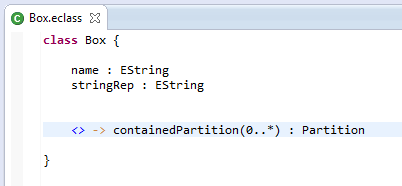
\includegraphics[width=0.6\textwidth]{eclass_box}
	\caption{Creating a \emph{contained reference} in \texttt{Box}}
	\label{fig:cpartitionReference}
\end{figure} 

\item[$\blacktriangleright$] Now add a \emph{simple reference} to \texttt{Partition}. Name it \texttt{box}, and allow it to hold up to one \texttt{Box}
(Fig.~\ref{fig:boxReference}). This means a single partition can belong to either zero, or one Box, and that is it. It can't belong to two different boxes at
the same time.

\begin{figure}[htbp]
	\centering
  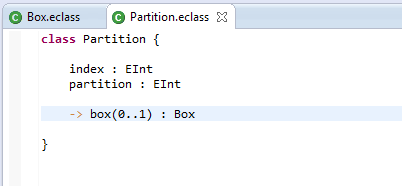
\includegraphics[width=0.6\textwidth]{eclass_partition}
	\caption{Creating a \emph{simple reference} in \texttt{Partition}}
	\label{fig:boxReference}
\end{figure} 

\item[$\blacktriangleright$] Congratulations, you have just built your first pair of EReferences. Together, this pair is also known as a \emph{Bidirectional
EReference}, since they connect their classes to eachother. To see how this is depicted visually, check out Fig.~\ref{fig:ereference_completed} in the previous
subsection.

\newpage

\item[$\blacktriangleright$] Now, lets create another bidirectional EReference between \texttt{Partition} and \texttt{Card}. If you think about it, it's really
not all that different than the relation between \texttt{Box} and \texttt{Partition}. In fact, it's not different at all! A \texttt{Partition} should be able
to hold an unlimited amount of \texttt{Card}s, but a \texttt{Card} should only be allowed to belong to zero or one \texttt{Partition}s. Name the two new
relations \texttt{containedPartition}, and \texttt{box}.

\item[$\blacktriangleright$] Your classes should now closely resemble Fig.~\ref{fig:almostAllReferences}.

\begin{figure}[htbp]
	\centering
  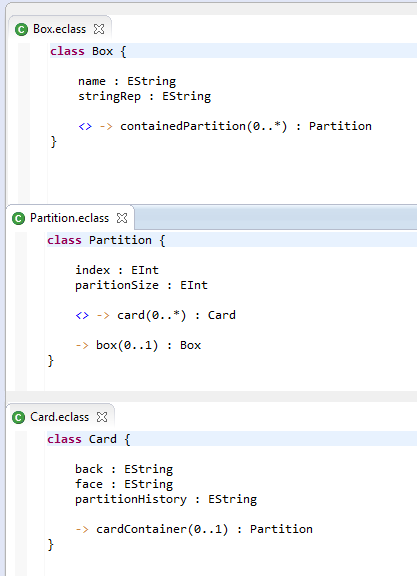
\includegraphics[width=0.65\textwidth]{eclipse_workspaceReferences}
	\caption{The Completed Bidirectional EReferences}
	\label{fig:almostAllReferences}
\end{figure} 

\item[$\blacktriangleright$] The next step is to set up two relations between \texttt{Partition} and itself, so it can shift between the previous and
next partition in the box. Create two new simple references, named \texttt{previous}, and \texttt{next}. Allow them to have a maximum of 1 link each.

\item[$\blacktriangleright$] If you have done everything correctly, your classes should now resemble Fig.~\ref{fig:allReferences}. 

\begin{figure}[htbp]
	\centering
  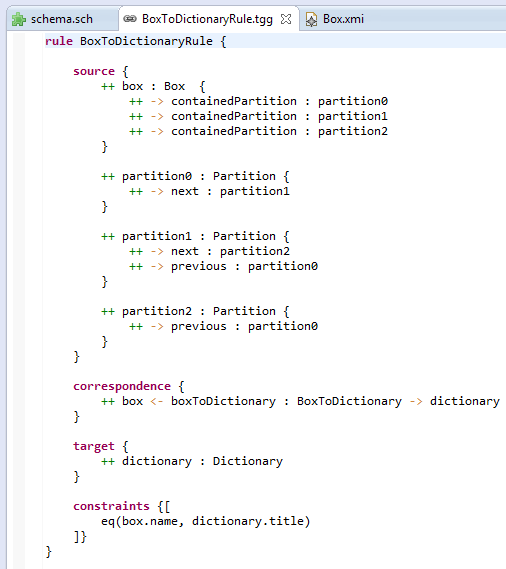
\includegraphics[width=0.6\textwidth]{eclipse_allReferences}
	\caption{All references in Leitner's Learning Box}
	\label{fig:allReferences}
\end{figure} 

\newpage

At this point, all of your references have been created! The problem is, suppose you set the \texttt{containedPartition} reference in a particular \texttt{Box}.
That's great, you would now have one box containing one partition. However, if you went and examined that partition independently, its \texttt{box} reference
would still be blank. We need to set up the link between these types so that when one updates, the other will be too.

\item[$\blacktriangleright$] Navigate to the ``\_constraints.mconf'' file. You can see it has a single \texttt{opposites} class that's currently empty. To
start, enter the following text: \texttt{containedPartition : Box <-> box : Partition}. This statement sets the two references to opposites of one another. 

% \item[$\blacktriangleright$] Your workspace should now resemble Fig.~\ref{fig:firstConstraint}.

% \begin{figure}[htbp]
% 	\centering
%   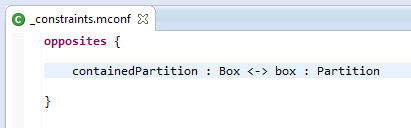
\includegraphics[width=0.6\textwidth]{eclipse_workspaceFirstConstraint}
% 	\caption{The first reference link}
% 	\label{fig:firstConstraint}
% \end{figure} 

\item[$\blacktriangleright$] Reviewing the \texttt{Partition} class, its easy to see that \texttt{previous} and \texttt{next} are not opposite to anything, but
we do need to establish the link between a \texttt{card} and its \texttt{cardContainer}. Follow the same steps until your workspace resembles
Fig.~\ref{fig:bothConstraints}.

\begin{figure}[htbp]
	\centering
  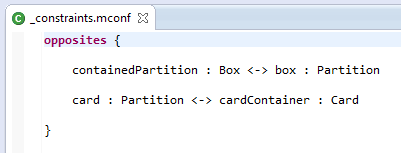
\includegraphics[width=0.6\textwidth]{eclipse_workspaceBothConstraints}
	\caption{The completed constraints file}
	\label{fig:bothConstraints}
\end{figure} 

\item[$\blacktriangleright$] Now the references for your Leitners learning box are truly complete! To see how each of the classes, attributes, and references
are depicted in the visual syntax, check out Fig.~\ref{fig:ereferences_all} in \hyperlink{sec:static vis}{section 2.1}. Otherwise, build your project to
make sure no errors exist, and continue to the next section to finalize the declaration of your classes.

\fancyfoot[R]{$\triangleright$ \hyperlink{static:methods tex}{Next}}

\end{itemize}
